\documentclass[a4paper]{article}
\usepackage[utf8]{inputenc}
\usepackage[T1]{fontenc}
\usepackage[french]{babel}
\usepackage{amsmath,amssymb}
\usepackage{amsfonts}
\usepackage{amssymb}
\usepackage{amsthm}
\usepackage{lmodern}
\usepackage{color}
\usepackage{graphicx}
\usepackage{geometry}
\usepackage{dialogue}


\def\dsum{\sum\limits}
\def\dint{\displaystyle\int}
\def\ie{\leqslant}
\def\C{\mathbb{C}}
 \parskip 5mm
 \parindent 5mm
 \definecolor{Green}{RGB}{20,200,50}
 \definecolor{Red}{RGB}{200,50,20}
 \definecolor{Blue}{RGB}{50,20,200}

 \geometry{top=15mm, bottom=15mm, left=17mm , right=17mm}

\author{\textcolor{Green}{The anonymous M. Maths}}
\title{\textcolor{Green}{\textbf{Probabilité et Statistiques}}}


\begin{document}
\maketitle
\tableofcontents
\newpage

\section{Petit Rappel}

\subsection{Définition}

\paragraph{}

\newtheorem{rappel}{Définition}
\begin{rappel}
 aussi  appelé  \textit{univers} et noté $\Omega$, est l'ensemble des résultats possibles associés à une expérience, on appelle ces éléments, "épreuves".
\end{rappel}

\textbf{Exemple :} L'ensemble fondamentale lié à \textbf{un} lancer de dé est {1,2,3,4,5,6} tandis que celui lié à \textbf{deux} lancer est \{1,2,3,4,5,6\} x \{1,2,3,4,5,6\} = \{(1,1),(1,2),(1,3),(1,4),(1,5),
\newline (1,6),(2,1),...,(6,6)\}, il s'agit du produit cartésiens des deux ensembles.
\vspace{5mm}
\begin{rappel}
La cardinalité d'un ensemble A noté \textit{Card(A)} ou \textit{|A|}, est le nombre d'élément de cette ensemble.
\end{rappel}

\textbf{Exemple :} Cardinal de l'ensemble {1,2,3,4,5,6} est 6 et celui de \{1,2,3,4,5,6\} x \{1,2,3,4,5,6\} est 6*6=36

\subsection{probabilité}

\subsubsection{{\underline{Formule:}}}
\paragraph{}
\begin{itemize}
\item P($\Omega$) = 1
\item P($\emptyset$) = 0
\item P(A) = $\dfrac{|A|}{|\Omega|}$
\item P($\overline{A}$) = 1 - P(A)
\item P(B--A) = P(B) -- P(B$\cap$A)
\item P(A$\cup$B) = P(A) + P(B) - P(A$\cap$B)
\item P(A$\cap$B) = P(A) + P(B) - P(A$\cup$B)


\end{itemize}

\subsubsection{{\underline{Probabilités conditionnelles:}}}

\paragraph{}
\textbf{Contexte :} M.Toutlemonde va au supermarché une et une seul fois par semaine soit le jeudi, soit le vendredi, soit le samedi. lorsqu'il va au supermarché, il va soit à SuperTimor\&Co soit à Motchane\&Motchane, le jeudi, il y a une chance sur 4 d'aller qu'il aille à superTimor\&Co, le vendredi, une chance sur 10 et le samedi 2 chances sur trois.
\newline On note respectivement J,V et S, les événements "M.Toutlemonde va au magasin le jeudi", "M.Toutlemonde va au magasin le vendredi", "M.Toutlemonde va au magasin le samedi"
\newline On note T, l'événement "M.Toutlemonde va à superTimor\&Co"

\paragraph{}

\begin{rappel}
La probabilité conditionnelle d'un événement A sachant B, noté \textit{P(A|B)} ou \textit{$\Pi$}, est la probabilité que A se réalise \textbf{en sachant que} B est réalisé.
\end{rappel}

\textbf{Exemple :} la phrase \textit{"lorsqu'il va au supermarché, il va soit à SuperTimor\&Co soit à Motchane\&Motchane, le jeudi, il y a une chance sur 4 d'aller qu'il aille à superTimor\&Co..."} définit la probabilité que M.Toutlemonde va à superTimer\&Co \textbf{en sachant qu'} il y va \textbf{le jeudi}. Il s'agit donc de la probabilité conditionnel de T sachant J $\rightarrow$ P(T|J)=1/4


\paragraph{}
\textbf{Formule:}
\begin{itemize}
\item P(A|B) = $\dfrac{P(A \cap B)}{P(B)}$
\item P(A $\cap$ B) = P(A) * P(B|A)
\item Formule de Bayes :P(A|B) = $\dfrac{P(B|A) * P(A)}{P(B)}$
\end{itemize}

\begin{rappel}
La probabilité totale d'un évènement A est la somme de tous les probabilités conditionnelles de A.
\end{rappel}

\newpage

\textbf{Exemple :} Si on s'interresse à la probabilité que M.Toutlemonde aille à superTimor\&Co dans la \textbf{semaine} il faut calculer la probabilités qu'il aille à superTimor\&Co le jeudi, le vendredi ou le samedi
Pour cela il faut faire la somme de la probabilités qu'il aille au supermarché le jeudi \textbf{et} à superTimer\&Co le jeudi plus celui qu'il aille au supermarché le vendredi \textbf{et} à superTimor\&Co le vendredi plus qu'il aille au supermarché le samedi \textbf{et} à superTimor\&Co le samedi.
\begin{dialogue}
\speak{M.Toutlemonde} Oulala, ça fait trop de probabilité
\speak{M.Maths} vous avez raison, un schéma vaut mieux que des mots
\newline
{\centering \resizebox{15cm}{10cm}{\includegraphics{prob_totale.png}}}
\newline
\speak{M.Maths} c'est plus claire?
\speak{M.Toutlemonde} si on veut...
\speak{M.Maths} pas très convaicant, en vert vous avez toutes les possibilités liés à l'événement je vais à superTimor\&Co $\rightarrow$ vous devez calculer la probabilité d'aller au magasin tel jour  et d'aller à superTimor\&Co ce jour là, et ceci pour chaque jour, puis les additionner, d'où l'expression probabilité totale.
\end{dialogue}

\textbf{Formule Général:}
P(A) = $\displaystyle{\sum_{i \in I} P(A|H_i) * P(H_i)}$

\subsubsection{{\underline{Indépendance:}}}

\begin{rappel}
Deux évènements A et B sont indépendant si l'un n'influe pas la probabilité de l'autre et inversement, autrement dit
P(A|B) = P(A) $\leftrightarrow$ P(A $\cap$ B)= P(A) * P(B)
\end{rappel}
\begin{dialogue}
\speak{M.Toutlemonde} ... et c'est tout?
\speak{M.Maths} ... euh ouai en fait c'est tout \newline par exemple l'événement M.Royaume-Uni se brosse les dents
et M.Toutlemonde va à superTimor\&Co sont indépendants, l'un n'influe pas sur l'autre, peu importe que M.Royaume-Uni se brosse les dents ou pas, la probabilité que M.Toutlemonde aille à superTimor\&Co ne change pas.
\speak{M.Toutlemonde} ah oui, en effet c'est tri...
\speak{M.Maths} ne prononcez pas ce mot s'il vous plaît
\end{dialogue}

\subsection{Coefficient binomial}

\begin{rappel}
Le coefficient binomial $C_n^k$, noté aussi ${n \choose k}$ permet de dénombrer toutes les combinaisons de k élément parmis n éléments en supposant que un même élément ne peut être retrouvé deux fois dans la même combinaison.
\end{rappel}

\textbf{Exemple :} l'exemple le plus illustrative est le jeu de carte. Admettons que nous jouons avec un jeu de 32 cartes
\newline $\rightarrow$ l'ensemble C des cartes \{coeur,trèfle,pique,carreau\} x \{as,7,8,9,10,vallet,reine,roi\}
\newline donc si vous avez bien suivi, ce produit cartésien forme l'ensemble des cartes composés, donc, de 8 coeurs, de 8 trèfles, 8 piques et 8 carreaux.
\newline je pioche maintenant 5 cartes, les combinaisons possibles sont C x C-\{la première carte\} x C-\{la première carte, la deuxième carte\} x C-\{la première carte, la deuxième carte, la troisième carte\} x C-\{la première carte, la deuxième carte, la troisième carte, la quatrième carte\}
Card($\Omega$) = 32 * 31 * 30 * 29 * 28 = $\dfrac{32!}{(32-5)!}$
Cependant, ici on parle d'arrangement $\rightarrow$, il s'agit d'une combinaison mais avec un ordre précis, l'ordre, ici, nous importe peu. Donc on doit enlevé les répétitions, pour cela on divise par le factorielle du nombre de cartes qu'on pioche, entre autre, ici, 5!.
\newline on obtient alors $\dfrac{32!}{5!(32-5)!}$, il s'agit de la formule du coeffiecient binomial $C_{32}^5$ (5 cartes parmis les 32 proposés)

\textbf{Formule Général:}$\displaystyle{{n \choose k} = \dfrac{n!}{k!(n-k)!}}$

\section{Variable aléatoire}

{\raggedright On dit que la variable aléatoire (v.a.) suit une loi lorsque la probabilité que celle ci soit égale à une valeur, est définis par la loi en question.\newline
\textbf{Exemple : X suit la loi définie ci-dessous}\par}
{\centering
\begin{tabular}{|c|c|c|c|c|}
\hline
x & 0 & 1 & 2 & 3 \\
\hline
P(X=x) & 0.1 & 0.5 & 0 & 0.4 \\
\hline
\end{tabular}
\par}
Dans ce tableau, on peut par exemple voir que la probabilité que la variable x soit égale à 1 est 50\%. 
\textit{Note:} La somme de toute les probabilités définis par une loi \textbf{ doit être égale à 1}
\newline
Si la loi de X est définis par une fonctions définis sur un ensemble E alors on dit que X est une variable aléatoire \emph{discrète finie} si E est un ensemble fini ( qui a des bornes) ou infinie si E est un ensemble infini dénombrable (au moins l'une des deux bornes est l'infini).
\subsection{Fonction de répartition}

La fonction de répartition de la variable aléatoire X est la fonction F tel que F(x) = P(X$\leq$x)
$$ P(X\leq x)= \sum_i^x P(X=i) \neq P(X>x)$$ 
$$P(X>x) = 1 - P(X\leq x)$$
Si on prend la loi précédente cela nous donne le tableau suivant
{\centering
\begin{tabular}{|c|c|c|c|c|}
\hline
x & 0 & 1 & 2 & 3 \\
\hline
$ F(x) = P(X \leq x) $ & 0.1 & 0.6 & 0 & 1 \\
\hline
\end{tabular}
\par}
\textit{Note:} Cette fonction de répartition est compris \textbf{dans l'intervale [0,1]}
\newline On peut aussi tracer son graphe à partir de ce Tableau.
\newline
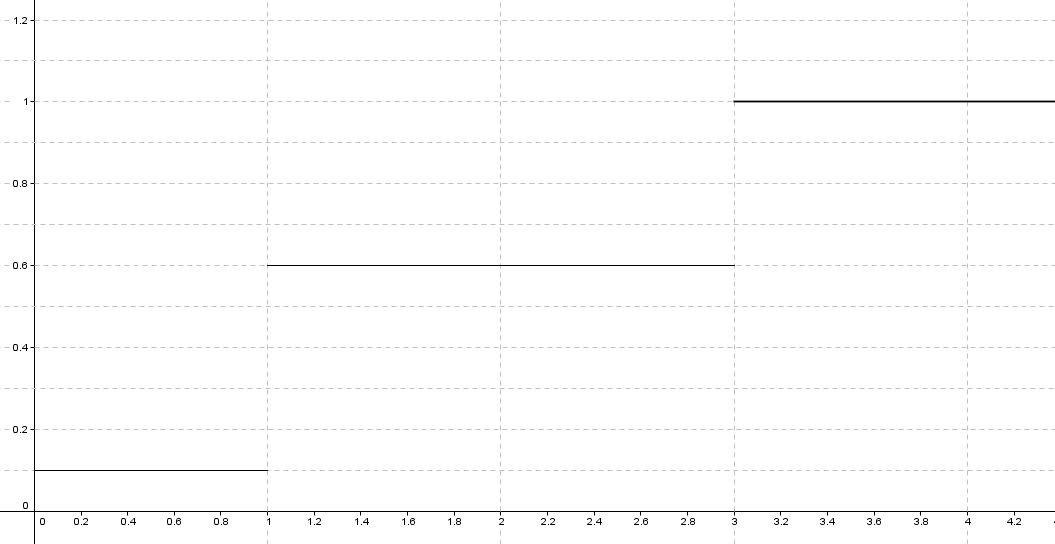
\includegraphics[scale=0.5]{Graph1.png}
\newline
ne vous amusez pas à dessiner des escaliers, cela peut vous être compter faux car on ne peut avoir de graphe vertical.

Maintenant supposons que X est une v.a discrète tel que 
\begin{eqnarray}
P(X=x) = f(x) = \left \{
\begin{array}{r c l}
0.1 x \text{ si 0$\leq x <4.5$} \\
0 \text{ sinon} \\
\end{array}
\right . 
\end{eqnarray}
\newline
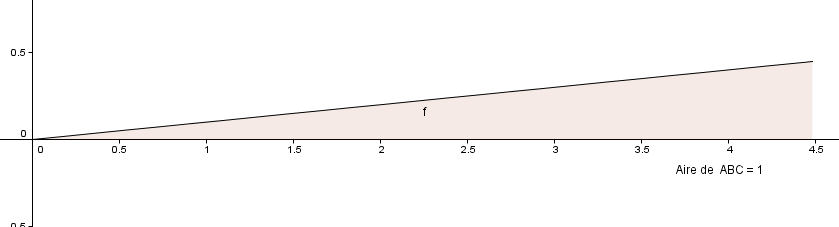
\includegraphics[scale=0.5]{Graph2.png}
\newline
Si je veux $P(X \leq 2)$ il faut que je calcul la somme de de tous les $f(i) = P(X=i)$ pour i inférieur à 2. Cela donne en fait l'aire entre la droite et l'axe x sur [0,2]
\newline
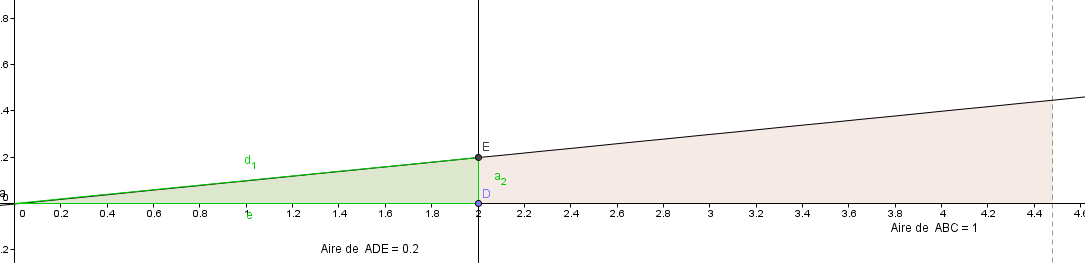
\includegraphics[scale=0.5]{Graph3.png}
\newline
Ce qui nous fais 0.2
\newline Ainsi pour calculer $P(X\leq x)$ quand x est inférieur à 4.5, il faut calculer l'intégrale sur [0,x], donc de $0.1x$,  ce qui nous donne ici $0.1x^2/2$. Puis sur [$-\infty$,0] ce qui nous donne 0 car la primitive de 0 c'est 0. On utilise alors la \textbf{relation de Chasle} qui consiste à additionner les différents aires sur [$-\infty$,x] (en somme, tout ce qui est inférieur à x) donc $P(X\leq x) = 0 \text{(integrale de f sur [$-\infty$,0])} + (F(x) - F(0)) \text{(integrale de f sur [0,x])} = 0 + 0.1 * x^2 /2 - 0.1 * 0 / 2 = 0.1 * x^2/2 \Leftrightarrow P(X \leq 2) = 0.2$ Donc \newline
\begin{eqnarray}
P(X\leq x) = F(x) = \left \{
\begin{array}{r c l}
0 \text{ si x$\leq 0$} \\
0.1 * x^2 / 2  \text{si $0<x \leq 2$} \\
1 \text{ sinon}
\end{array}
\right . 
\end{eqnarray}

\textbf{Propriété :} La fonction de répartition d'une variable discrète X tel que f(x) = P(X=x) est la primitive de la fonction f dans si et seulement si, à l'intérieur des bornes dans laquelle elle est définis :
\begin{itemize}
\item f et continue à l'intérieur des bornes dans laquelle elle est définis
\item f est positif 
\item L'intégrale de f, de sa borne inférieur à sa borne supérieur, est égale à 1
\end{itemize} 
On dit alors que X est une v.a continue et que f est sa densité de probabilité ($\neq$ fonction de répartition)
Dans notre exemple, la fonction f est continue et positif sur [$-\infty , +\infty$] et 
$$ \int_{-\infty}^{+\infty} f(t)\text{d}t = li - F(0) = 1 $$
donc f(x) est la densité de probabilité de X. \textbf{Attention}, sa fonction de répartition n'est pas 

\subsection{Couple de variable Aléatoire}

La loi du couple des variables aléatoires X,Y est la loi $P_{XY}$ tel que $P_{XY}({(x,y)})$ soit la probabilité que X soit égale à x et Y soit égale à y. On le note plus communément $P(X=x \bigcap Y=y)$. \newline
\textbf{Exemple :} Le couple (X,Y) suit la loi suivante : \newline
\begin{tabular}{|c|c|c|c|}
\hline
x / y & 0 & 1 & P(X = x)\\
\hline
0 & \textcolor{Blue}{0.3} & 0.1 & 0.4\\
\hline
1 & 0.15 & 0.2 & 0.35 \\
\hline
2 & 0.1 & 0.15 & \textcolor{Green}{0.25}\\
\hline
P(Y=y) & \textcolor{Red}{0.55} & 0.45 & 1\\
\hline
\end{tabular}
\newline
J'ai ici utilisé la formule des probabilités totales pour calculer la ligne P(Y=y) et la colonne P(X=x).
\begin{itemize}
\item La case blue est la probabilité $P(X=0 \bigcap Y=0)$. 
\item La case verte est la probabilité $P(X=2)$. 
\item La case rouge est la probabilité $P(Y=0)$. 
\end{itemize}
\subsection{Loi usuelle}
Les lois usuelles sont des lois qui sont appliqués à une certaine situation et sont définis par certaines règles.
\subsubsection{Loi}

\end{document} 